\documentclass[aspectratio=169]{../latex_main/tntbeamer}  % you can pass all options of the beamer class, e.g., 'handout' or 'aspectratio=43'
\usepackage{dsfont}
\usepackage{bm}
\usepackage[english]{babel}
\usepackage[T1]{fontenc}
%\usepackage[utf8]{inputenc}
\usepackage{graphicx}
\graphicspath{ {./figures/} }
\usepackage{algorithm}
\usepackage[ruled,vlined,algo2e,linesnumbered]{algorithm2e}
\usepackage{hyperref}
\usepackage{booktabs}
\usepackage{mathtools}

\usepackage{amsmath,amssymb}

\DeclareMathOperator*{\argmax}{arg\,max}
\DeclareMathOperator*{\argmin}{arg\,min}

\usepackage{amsbsy}
\newcommand{\vect}[1]{\bm{#1}}
%\newcommand{\vect}[1]{\boldsymbol{#1}}

\usepackage{pgfplots}
\pgfplotsset{compat=1.16}
\usepackage{tikz}
\usetikzlibrary{trees} 
\usetikzlibrary{shapes.geometric}
\usetikzlibrary{positioning,shapes,shadows,arrows,calc,mindmap}
\usetikzlibrary{positioning,fadings,through}
\usetikzlibrary{decorations.pathreplacing}
\usetikzlibrary{intersections}
\pgfdeclarelayer{background}
\pgfdeclarelayer{foreground}
\pgfsetlayers{background,main,foreground}
\tikzstyle{activity}=[rectangle, draw=black, rounded corners, text centered, text width=8em]
\tikzstyle{data}=[rectangle, draw=black, text centered, text width=8em]
\tikzstyle{myarrow}=[->, thick, draw=black]

% Define the layers to draw the diagram
\pgfdeclarelayer{background}
\pgfdeclarelayer{foreground}
\pgfsetlayers{background,main,foreground}

% Requires XeLaTeX or LuaLaTeX
%\usepackage{unicode-math}

\usepackage{fontspec}
%\setsansfont{Arial}
\setsansfont{RotisSansSerifStd}[ 
Path=../latex_main/fonts/,
Extension = .otf,
UprightFont = *-Regular,  % or *-Light
BoldFont = *-ExtraBold,  % or *-Bold
ItalicFont = *-Italic
]
\setmonofont{Cascadia Mono}[
Scale=0.8
]

% scale factor adapted; mathrm font added (Benjamin Spitschan @TNT, 2021-06-01)
%\setmathfont[Scale=1.05]{Libertinus Math}
%\setmathrm[Scale=1.05]{Libertinus Math}

% other available math fonts are (not exhaustive)
% Latin Modern Math
% XITS Math
% Libertinus Math
% Asana Math
% Fira Math
% TeX Gyre Pagella Math
% TeX Gyre Bonum Math
% TeX Gyre Schola Math
% TeX Gyre Termes Math

% Literature References
\newcommand{\lit}[2]{\href{#2}{\footnotesize\color{black!60}[#1]}}

%%% Beamer Customization
%----------------------------------------------------------------------
% (Don't) Show sections in frame header. Options: 'sections', 'sections light', empty
\setbeamertemplate{headline}{empty}

% Add header logo for normal frames
\setheaderimage{
	% 
\includegraphics[height=\logoheight]{figures/TNT_darkv4.pdf}
	
\includegraphics[height=\logoheight]{../latex_main/figures/luh_logo_rgb_0_80_155.pdf}
	% 
\includegraphics[height=\logoheight]{figures/logo_tntluh.pdf}
}

% Header logo for title page
\settitleheaderimage{
	% 
\includegraphics[height=\logoheight]{figures/TNT_darkv4.pdf}
	
\includegraphics[height=\logoheight]{../latex_main/figures/luh_logo_rgb_0_80_155.pdf}
	% 
\includegraphics[height=\logoheight]{figures/logo_tntluh.pdf}
}

% Title page: tntdefault 
\setbeamertemplate{title page}[tntdefault]  % or luhstyle
% Add optional title image here
%\addtitlepageimagedefault{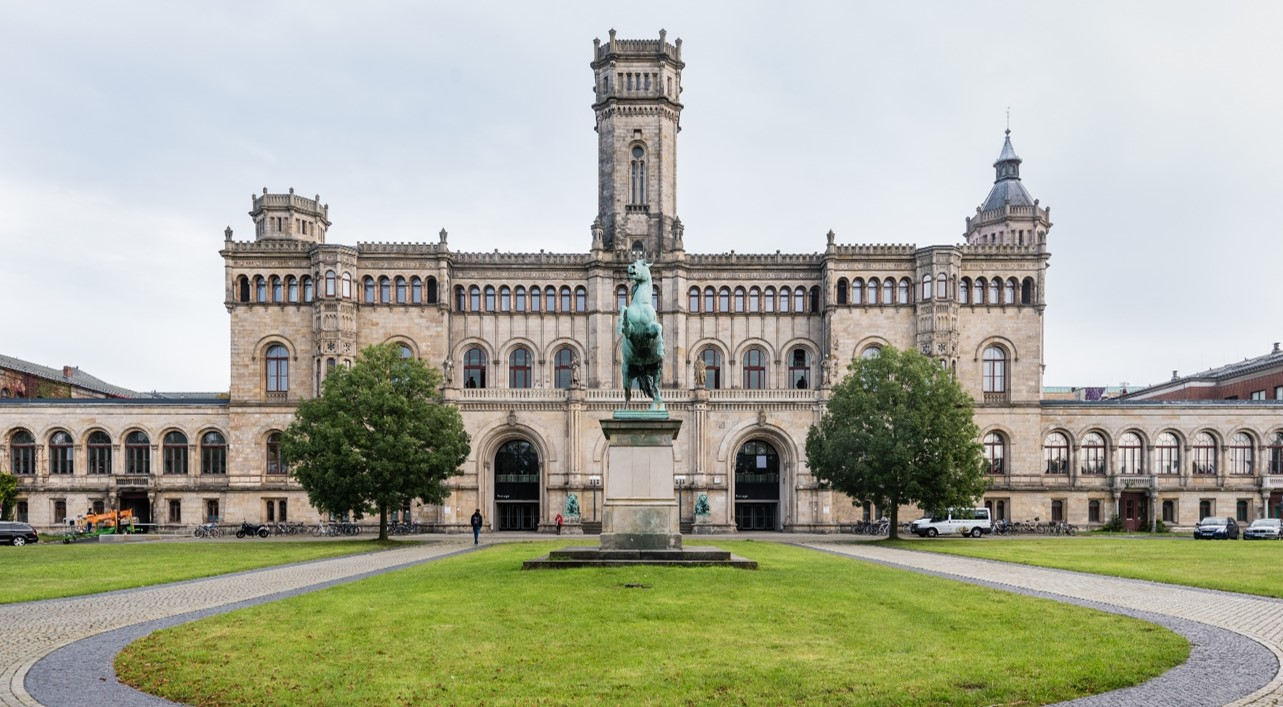
\includegraphics[width=0.65\textwidth]{figures/luh_default_presentation_title_image.jpg}}

% Title page: luhstyle
% \setbeamertemplate{title page}[luhstyle]
% % Add optional title image here
% \addtitlepageimage{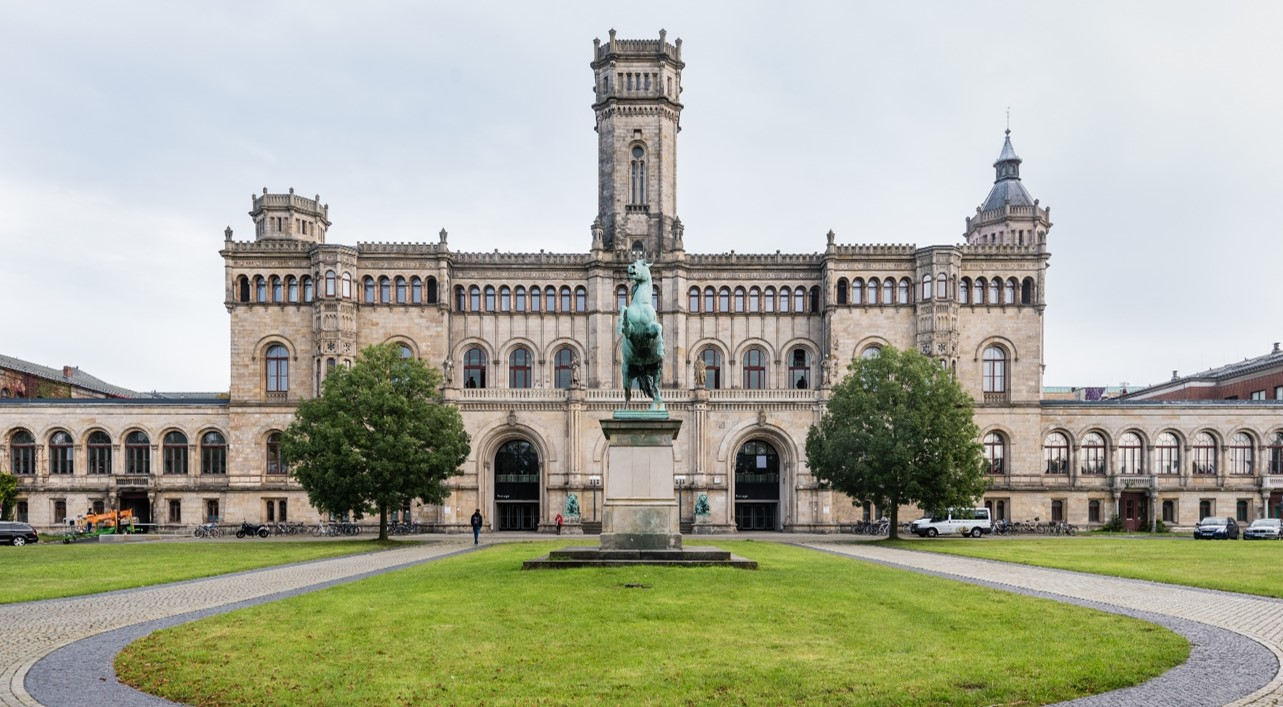
\includegraphics[width=0.75\textwidth]{figures/luh_default_presentation_title_image.jpg}}

\author[Abedjan \& Lindauer]{Ziawasch Abedjan \& Marius Lindauer\\[1em]
	
\includegraphics[height=\logoheight]{../latex_main/figures/luh_logo_rgb_0_80_155.pdf}\qquad
	
\includegraphics[height=\logoheight]{../latex_main/figures/DBIS_Kurzlogo.png}\qquad

\includegraphics[height=\logoheight]{../latex_main/figures/TNT_darkv4}\qquad

\includegraphics[height=\logoheight]{../latex_main/figures/L3S.jpg}	}
\date{Summer Term 2022; \hspace{0.5em} {
\includegraphics[height=1.5em]{../latex_main/figures/Cc-by-nc-sa_icon.svg.png}}; based on \href{https://ds100.org/fa21/}{[DS100]}
}


%%% Custom Packages
%----------------------------------------------------------------------
% Create dummy content
\usepackage{blindtext}

% Adds a frame with the current page layout. Just call \layout inside of a frame.
\usepackage{layout}


%%% Macros
%\renewcommand{\vec}[1]{\mathbf{#1}}
% \usepackage{bm}
%\let\vecb\bm

\title[Introduction]{DS: Data Sampling and Probability}
\subtitle{Binomial and multinomial probabilities}

\graphicspath{ {./figure/} }
%\institute{}


\begin{document}
	
	\maketitle
	
	
	\begin{frame}{The scenario}
	Binomial and multinomial probabilities arise when we:
	\begin{itemize}
	    \item Sample at random, with replacement.
	    \item Sample a fixed number (n) times.
	    \item Sample from a categorical distribution.
	    \begin{itemize}
	        \item For example, a bag of marbles in which 60\% are blue and 40\% are not blue.
	        \item Or where 60\% are blue, 30\% are green, and 10\% are red.
	    \end{itemize}
	    \item Want to count the number of each category that end up in our sample.
	\end{itemize}
	    Note: In this section, we will make use of the binomial coefficient and factorials. If you want a refresher on these, or want a more in-depth understanding, there’s an extra section at the end of this lecture that covers the derivation and some examples of it.

	\end{frame}
	
	
	\begin{frame}{Two categories}
	Suppose we sample at random with replacement 7 times from a bag of marbles, 60\% of which are blue and 40\% of which are not blue.

	\begin{itemize}
	    \item What is P(bnbbbnn)?
	    \begin{itemize}
	        \item By the product rule from Data 8, since the sample is drawn with replacement:
            \begin{align*}
                P(bnbbbnn) &= 0.6 \times 0.4 \times 0.6 \times 0.6 \times 0.6 \times 0.4 \times 0.4 \\
                &= (0.6)^4 (0.4)^3
            \end{align*}
	    \end{itemize}
	    \item How does P(4 blue, 3 not blue) compare to P(bnbbbnn)?
	    \begin{itemize}
	        \item P(4 blue, 3 not blue) > P(bnbbbnn).
	        \item Why? bnbbbnn is far more restrictive and specific than “4 blue, 3 not blue.”
	        \item There are several other ways to get “4 blue, 3 not blue” (for instance, bnnnbbb).
	    \end{itemize}
	\end{itemize}

	\end{frame}
	
	
		\begin{frame}{Binomial probabilities...}
	“4 blue, 3 not blue” can occur in several equally likely ways.\\                     For instance, P(bnbbbnn) = P(bnbbbnn) = P(bnbbbnn) = ... = $(0.6)^4$ $(0.4)^3$. \\         \bigskip
	    
	    P(4 blue, 3 not blue) is the total chance of all of those ways. The number of ways in which we can draw 4 blue marbles and 3 not blue marbles is

        \begin{align*}
            \binom{7}{4} = \frac{7!}{4!3!}
        \end{align*}
    and thus,
    \begin{align*}
        \text{P(4 blue, 3 not blue)} = \binom{7}{4}(0.6)^4 (0.4)^3 = \frac{7!}{4!3!}(0.6)^4 (0.4)^3
    \end{align*}

	\end{frame}
	
	
	\begin{frame}{Next time: random variables}
    	\begin{itemize}
    	    \item In the next lecture, we will formalize the notion of a random variable. Random variables arise naturally from this notion of a sample.
    	    \item We will then explore properties of random variables. 
    	    \begin{itemize}
    	        \item Expectation and variance.
    	        \item Various distributions.
    	        \item Sample means and sums.
    	    \end{itemize}
    	    \item We will then take a break from this discussion on sampling and probability, and switch gears to some of the more tools-focused ideas in this class. 
    	    \begin{itemize}
    	        \item SQL, pandas, regex, visualization, etc.
    	    \end{itemize}
    	    \item But not to worry – sampling, probability, and random variables in particular will reappear later in the semester.
    	\end{itemize}

	\end{frame}

\end{document}